\documentclass{beamer}
\usepackage{lipsum}
\usepackage[brazilian]{babel}
\usepackage[utf8]{inputenc}

\usepackage{enumerate}
\usepackage{dcolumn}
\usepackage{tabu}
\usepackage{colortbl}
\usepackage{booktabs}
\usepackage{changes}
\usepackage{listings}
\usepackage{placeins}
\usepackage{amsmath}

\usepackage{multirow}

\newcommand*{\Scale}[2][4]{\scalebox{#1}{$#2$}}%
\newcommand*{\Resize}[2]{\resizebox{#1}{!}{$#2$}}%

\usetheme[faculty=ppca,language=logo,framenumber,totalframenumber]{UniversiteitGent}

\title{Desenvolvimento de Microserviços \\ no CPD/UnB }
\subtitle{ \textcolor{forestgreen}{Universidade de Brasília} \\
			\textcolor{black}{Centro de Informática} \\
			4 de Dezembro de 2017
}
\author{Everton de Vargas Agilar \\
		evertonagilar@unb.br
}



\begin{document}

\begin{frame}
  \titlepage
\end{frame}




%%##############################################################




\subsection{Plan}

\begin{frame}
  \frametitle{Plano}

    \begin{itemize}

	    \item<1-> Nova Arquitetura de Desenvolvimento do CPD/UnB
		    \begin{itemize}
				\item<1->Motivação para adoção de SOA
				\item<1->Ferramentas e tecnologias adotadas e desenvolvidas
				\item<1->ErlangMS -- Plataforma agnóstica de serviços
			\end{itemize}

  	  	\item<1-> Implementação de Serviços e Microserviços
		    \begin{itemize}
				\item<1->Desenvolvimento de serviços em Java
				\item<1->Autenticação de usuários com o proxy LDAP
				\item<1->Autenticação e autorização de serviços REST com OAuth2
  		     \end{itemize}
 	  
	   	\item<1-> Trabalhos Futuros
	   	  
    \end{itemize}

\end{frame}



\begin{frame}
\frametitle{Motivação para adoção de SOA}

\begin{itemize}
	\item<1->Maximizar o reuso dos fluxos de negócios;
	\item<1->Modernizar os sistemas de maneira sistemática e incremental;
	\item<1->Minimizar dependências tecnológicas; 
	\item<1->Experimentar SOA (Service Oriented Architecture).
\end{itemize}

\end{frame}


\begin{frame}
\frametitle{Ferramentas e tecnologias adotadas}

\begin{figure}
	\centering
	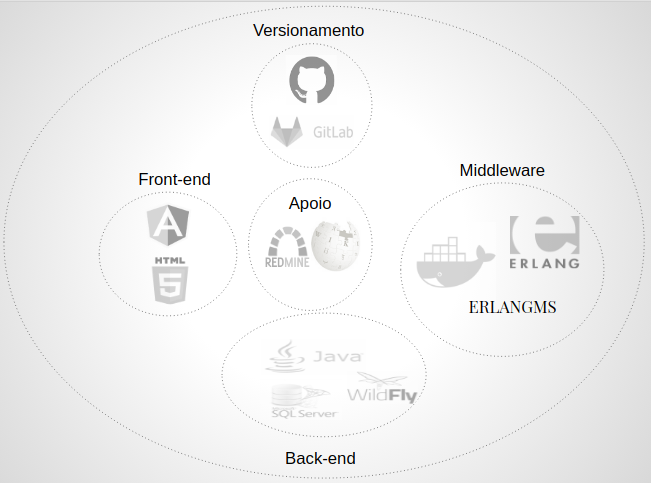
\includegraphics[scale=0.25]{img/tec.png}
\end{figure}

\end{frame}


%%##############################################################




\section{Introdução}


\subsection{Introdução}


%%##############################################################




\subsection{Sobre}


\begin{frame}
  \frametitle{ErlangMS -- Plataforma agnóstica de serviços}

  \begin{exampleblock}{ERLANGMS}
  
É uma plataforma de software desenvolvida para facilitar a integração de sistemas por meio de um barramento 
de serviços orientado a contratos de serviços + SDK + Processo de modernização e arquitetura documentado (SMSOC).

  \end{exampleblock}

  
\end{frame}


\begin{frame}
  \frametitle{ErlangMS -- Plataforma agnóstica de serviços}

  \begin{exampleblock}{Características do barramento}
  
	  \begin{itemize}
		\item<1->Multiplataforma e arquitetura modular;
	    \item<1->Serviços especificados em catálogos de serviços;
	    \item<1->Suporta serviços RESTful com alta escalabilidade;
   	    \item<1->Modelo de concorrência: Actor Model;
   	    \item<1->Integração com SGBD via ODBC e Data loaders;
		\item<1->Implementação de web services em Erlang e Java
	  \end{itemize}

  \end{exampleblock}

  
\end{frame}


\begin{frame}
  \frametitle{ErlangMS -- Plataforma agnóstica de serviços}

  \begin{exampleblock}{Características do barramento}
  
	  \begin{itemize}
		\item<1->HTTP/2, HTTP/1.1, HTTPS (Secure TLS Listener);
	    \item<1->LDAP v3 -- Proxy LDAP;
	    \item<1->HTTP Basic authentication;
    	    \item<1->OAuth2 authentication;
		\item<1->Api query -- filter, fields, sort, limit.
	  \end{itemize}

  \end{exampleblock}

  
\end{frame}


  
\end{frame}




%%##############################################################



\section{Principais Resultados do Trabalho}


\begin{frame}[c]{ }
\centering
  \huge{Principais Resultados do Trabalho}
\end{frame}



\begin{frame}
  \frametitle{Desenvolvimento de serviços em Java}

	\begin{figure}
	\centering
		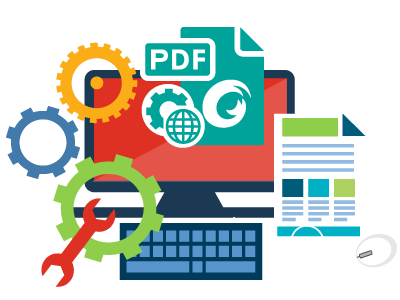
\includegraphics[scale=0.4]{img/sdk.png}
	\end{figure}
  
\end{frame}


\begin{frame}
  \frametitle{Autenticação de usuários com o proxy LDAP}

	\begin{figure}
	\centering
		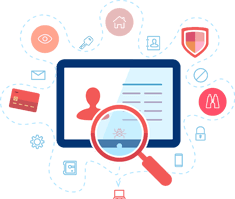
\includegraphics[scale=0.6]{img/ldap.png}
	\end{figure}
  
\end{frame}


\begin{frame}
  \frametitle{Autenticação e autorização de serviços REST com OAuth2}

	\begin{figure}
	\centering
		
\includegraphics[scale=0.4]{img/oauth2.png}
	\end{figure}
  
\end{frame}



\begin{frame}
  \frametitle{Trabalhos futuros}

  \begin{exampleblock}{Trabalhos futuros}
  
	  \begin{itemize}
 	    \item<1->Portal Api Management;
    	    \item<1->JSON Schema Draft 4;
    	    \item<1->SDK .Net.
	  \end{itemize}

  \end{exampleblock}

  
\end{frame}


%%##############################################################


\subsection{Perguntas}


\begin{frame}[c]{ }
\centering
  \huge{Perguntas ?}
\end{frame}


\begin{frame}
  \frametitle{Perguntas}

  \begin{exampleblock}{}
  
	  \begin{itemize}
		\item<1->(QP1) Por que Erlang/OTP?
		\item<1->(QP2) Quem usa Erlang/OTP?
	    \item<1->(QP3) Por que o desenvolvimento de um novo barramento em vez de utilizar um existente?
	    \item<1->(QP4) Por que não implementar web services usando somente Java e seus frameworks?
	  \end{itemize}
  
  \end{exampleblock}

  
\end{frame}


\begin{frame}
  \frametitle{(QP1) Por que Erlang/OTP?}

    \begin{itemize}
       \item<1-> Suporta aplicações distribuídas e tolerantes a falhas a serem executadas em um ambiente de tempo real e ininterrupto;
       \item<1-> Possui um ambiente de execução que realmente facilita o desenvolvimento de software de rede e de clusters de serviços;
       
       \item<1-> Possui um modelo de arquitetura baseado em atores (Actor Model) onde os processos podem 
       se comunicar apenas por mensagens.
       
    \end{itemize}
  
\end{frame}


\begin{frame}
  \frametitle{(QP2) Quem usa Erlang/OTP?}

	  \begin{itemize}
		\item<1->Facebook (Backend do chat -- 100 milhões de usuários ativos);
		\item<1->Whatapps (Servidores de mensagens -- 2 milhões de usuários/servidor);
		\item<1->Yahoo (Delicious -- 5 milhões de usuários e mais de 150 milhões de bookmarks);
		\item<1->Amazon SimpleDB, o serviço de dados do Amazon EC2;
		\item<1->GitHub (Backend -- milhares de transações concorrentes);
		\item<1->T-Mobile nos seus sistemas de SMS e autenticação;
		\item<1->Motorola, CouchDB, RabbitMQ, Ejabbed, entre outros.
						
	   \end{itemize}
  
\end{frame}


\begin{frame}
  \frametitle{(QP3) Por que um novo barramento?}

	  \begin{itemize}
		\item<1->Obter domínio sobre as tecnologias e o design RESTful;
		\item<1->Barramento de serviços são produtos caros e complexos;
		\item<1->Disponibilizar um produto simples (contém somente 10 mil linhas de código atualmente).
					
	   \end{itemize}
  
\end{frame}


\begin{frame}
  \frametitle{(QP4) Por que não implementar web services em Java com frameworks?}

	  \begin{itemize}
		\item<1->É uma opção, mas exige ferramentas para gerenciar;
		\item<1->Não é orientado a contrato de serviços;
		\item<1->Não é independente de linguagem de programação;
		\item<1->Não é escalável apenas usando os frameworks.
	   \end{itemize}
  
\end{frame}



\begin{frame}[c]{ }
\centering
  \huge{Obrigado!}
\end{frame}


\end{document}



